\documentclass[10pt]{article}

% Preprint option: author visible, no ``under review'' banner, no claim of publication.
\usepackage[preprint]{tmlr}

\usepackage{amsmath,amssymb,amsthm,mathtools,booktabs,graphicx,microtype,hyperref}
\newtheorem{proposition}{Proposition}

\title{Convergence of the Brier Score,\\ a Weighted Squared Divergence, and\\ Kullback--Leibler Divergence}

\author{\name Brando Miranda \email brando9@stanford.edu \\
  \addr Department of Computer Science\\
  Stanford University}

\def\month{11}
\def\year{2026}

\newcommand{\R}{\mathbb{R}}
\newcommand{\BS}{\mathrm{BS}}
\newcommand{\WD}{\mathrm{WD}}
\newcommand{\KL}{\mathrm{KL}}

\begin{document}
\maketitle

\begin{abstract}
We compare three objectives for a forecast $q$ on a finite alphabet, when the outcome is drawn from a distribution $p$: the Brier score, the weighted squared divergence $\WD(p,q)=\sum_a p(a)\bigl(p(a)-q(a)\bigr)^2$, and Kullback--Leibler divergence $\KL(p\|q)$.
First, substituting a one-hot distribution into the weighted squared divergence produces $(1-q(x))^2$, the local square score, and that score is not the Brier score.
Second, all three objectives are uniquely minimized at $q=p$, but their local rates on the probability simplex differ: the Brier score has rate $2$ in every tangent direction, the weighted squared divergence has rates proportional to $p(a)$, and Kullback--Leibler divergence has rates proportional to $1/p(a)$.
Third, log loss is local, so one outcome does not depend on how the remaining probability is split, while $\KL(p\|q)$ still diverges if any in-support coordinate of $q$ reaches $0$.
The same singularity makes the probability-space gradient large, which is why the local log score is not slow.
Finally, in softmax logit coordinates the gradient of expected log loss is $q-p$ and stays bounded, and it revives a class whose logit has collapsed; the Brier score and the weighted squared divergence do not, on the horizons we integrate, because their logit gradients are multiplied by the collapsed probability.
There is no smooth local proper score whose probability-space gradient stays bounded on the whole simplex.
\end{abstract}

\section{Introduction}

A forecast on a finite alphabet is a vector $q$ in the probability simplex.
The notes this report comes from asked whether the Brier score and a weighted squared divergence converge to the same forecast at different rates, and then asked a second question: log loss is local, so why is it not slow, and can it be made as stable as the Brier score by penalizing symbols that did not occur?

The mathematical content of those questions is short.
The Brier score of an outcome $x$ is the squared Euclidean distance between $q$ and the one-hot vector at $x$ \citep{brier1950}.
The weighted squared divergence puts an extra factor $p(a)$ on each coordinate of that distance between two distributions.
Those are different functions.
Both are uniquely minimized at the true distribution, and the extra factor $p(a)$ is exactly a slower local rate on rare symbols.
The expression obtained by substituting a one-hot vector into the weighted squared divergence keeps only the observed coordinate.
That expression is local, like log loss \citep{good1952}, and for an alphabet of size at least $3$ it is not proper \citep{bernardo1979,mit67800}.

Log loss then looks like a puzzle.
A local score does not look at the probabilities of the symbols that failed to occur.
The weighted squared divergence is slow on rare symbols because its gradient carries $p(a)$.
Log loss is local and yet, in the flows below, faster than the Brier score near the truth.
The resolution is that locality of the scalar loss and flatness of the population objective are different properties.
Expected log loss still depends on every coordinate, through the distribution of which symbol occurs, and its derivative in coordinate $a$ is $-p(a)/q(a)$.
A coordinate that is too small produces a large derivative.
The identity $-\log 0 = +\infty$ is that fact written as a barrier: it is real, it is stronger than the Brier score's finite penalty, and it is why the flow does not stall on the boundary the way the local square score does.

We make the following contributions:
\begin{enumerate}
\item We separate the Brier score, the weighted squared divergence, and the local square score, and we record which of them are proper.
\item We give the local rates of the three population objectives on the simplex and measure the corresponding gradient flows.
\item We separate the two penalties that the question about zero mixes up: the split of probability among symbols that did not occur, and the barrier at zero probability on a symbol that can occur.
\item We show that the softmax parameterization makes the log-loss gradient bounded without adding an unobserved-symbol penalty, and that a collapsed class is revived by that gradient and not by the Brier score on the same horizon.
\item We show that the repairs which keep log loss local move the minimizer, while a nonnegative multiple of the Brier score does not.
\end{enumerate}

\section{Three objectives}
\label{sec:defs}

Let $\mathcal{X}$ be a finite alphabet with $K=|\mathcal{X}|\ge 2$, and let $\Delta$ be the probability simplex $\{q\in\R^K: q\ge 0,\ \sum_a q(a)=1\}$.
The true distribution $p\in\Delta$ has full support unless we say otherwise.
The one-hot vector at an outcome $x$ is $e_x$.

The \emph{Brier score} of a forecast $q\in\Delta$ on outcome $x$ is
\begin{equation}
\label{eq:brier}
\BS(q,x) = \|q-e_x\|_2^2 = \bigl(1-q(x)\bigr)^2 + \sum_{a\neq x} q(a)^2.
\end{equation}
The population Brier objective is $R_{\BS}(q)=\mathbb{E}_{X\sim p}[\BS(q,X)]$.

The \emph{weighted squared divergence} compares the two distributions inside an expectation under $p$:
\begin{equation}
\label{eq:wd}
\WD(p,q)
= \sum_a p(a)\bigl(p(a)-q(a)\bigr)^2
= \mathbb{E}_{X\sim p}\bigl[(p(X)-q(X))^2\bigr].
\end{equation}
The summand is the squared difference of the probability values $p(X)$ and $q(X)$.
Evaluating it requires $p$, or a histogram substituted for $p$.
The outcome index does not determine the value $p(X)$, so one sample of $X$ does not determine the summand.

\emph{Log loss} of one outcome is $\ell(q,x)=-\log q(x)$, for $q(x)>0$.
\emph{Expected log loss} is $R_{\log}(q)=\mathbb{E}[-\log q(X)]$.
\emph{Kullback--Leibler divergence} is the same expectation with the log-likelihood ratio in place of the square:
\begin{equation}
\label{eq:kl}
\KL(p\|q)
= \mathbb{E}_{X\sim p}\bigl[\log p(X)-\log q(X)\bigr]
= R_{\log}(q) - H(p),
\end{equation}
where $H(p)=-\sum_a p(a)\log p(a)$ does not depend on $q$.
Gradients and minimizers of $R_{\log}$ and of $\KL(p\|q)$ therefore agree.
We report flows of $\KL(p\|q)$ and one-sample updates of log loss.
The one-sample update is log loss.
Expected log loss differs from Kullback--Leibler divergence by the constant $H(p)$.

Both divergences have the form $\mathbb{E}_{X\sim p}[d(p(X),q(X))]$.
For the weighted squared divergence, $d(u,v)=(u-v)^2$.
For Kullback--Leibler divergence, $d(u,v)=\log u-\log v$.
Substituting $p=e_x$ collapses each expectation to the observed atom.
The square becomes $(1-q(x))^2$, the local square score defined in Section~\ref{sec:identity}.
The log-likelihood ratio becomes $-\log q(x)$, which is log loss.
On $p=(0.70,0.20,0.10)$ and $q=(0.05,0.90,0.05)$ the two expectations equal $0.394$ and $1.616$.
Their Euclidean gradients there are $2p\odot(q-p)=(-0.91,0.28,-0.01)$ and $-p/q=(-14,-2/9,-2)$.
One sample of log loss on the first symbol has partial derivative $(-20,0,0)$.

A score $S(x,q)$ is \emph{local} when it depends on the forecast only through the scalar $q(x)$ \citep{mit67800}.
It is \emph{proper} when, for every $p\in\Delta$, the expectation $\mathbb{E}_{X\sim p}[S(X,q)]$ is uniquely minimized at $q=p$.
Log loss is local and proper \citep{good1952,bernardo1979}.
The Brier score is proper and not local \citep{brier1950,gneiting2007}.
For $K\ge 3$, every smooth local proper score is an affine image of log loss, $S(x,q)=-A\log q(x)+B(x)$ with $A>0$ \citep{bernardo1979,mit67800}.

\section{The local square score is not the Brier score}
\label{sec:identity}

Substituting $p=e_x$ into \eqref{eq:wd} deletes every term except $a=x$:
\begin{equation}
\label{eq:local-square}
\WD(e_x,q) = \bigl(1-q(x)\bigr)^2.
\end{equation}
Call the right-hand side the \emph{local square score}.
Equation \eqref{eq:brier} says the Brier score is the local square score plus $\sum_{a\neq x} q(a)^2$.
The second sum is zero only when $q$ puts no mass on the symbols that did not occur.
On $200$ random forecasts with $K$ drawn from $2$ through $7$, that gap was as large as $0.952$.

The unweighted squared distance $\sum_a\bigl(p(a)-q(a)\bigr)^2$ does not have this problem.
Substituting $p=e_x$ recovers \eqref{eq:brier}.
The extra weight $p(a)$ in \eqref{eq:wd} is the whole difference between the two derivations.

\begin{proposition}
\label{prop:brier-pop}
$R_{\BS}(q)=\|q-p\|_2^2+\sum_a p(a)\bigl(1-p(a)\bigr)$.
The unique minimizer on $\Delta$ is $q=p$.
\end{proposition}

\begin{proof}
$\|q-e_X\|_2^2=\|q\|_2^2+1-2q(X)$.
Taking the expectation gives $\|q\|_2^2+1-2\langle q,p\rangle=\|q-p\|_2^2+1-\|p\|_2^2$, and $1-\|p\|_2^2=\sum_a p(a)\bigl(1-p(a)\bigr)$.
The first summand is nonnegative and zero only at $q=p$.
\end{proof}

\begin{proposition}
\label{prop:wd}
If $p$ has full support, $\WD(p,q)=0$ if and only if $q=p$, so $q=p$ is the unique minimizer of \eqref{eq:wd} on $\Delta$.
\end{proposition}

\begin{proof}
Each summand is nonnegative, and $p(a)>0$ forces $q(a)=p(a)$.
\end{proof}

\begin{proposition}
\label{prop:local-square}
The local square score is proper when $K=2$.
When $K\ge 3$ it is not proper.
\end{proposition}

\begin{proof}
For $K=2$, write $q=(t,1-t)$ and $p=(\pi,1-\pi)$.
The expected score is $\pi(1-t)^2+(1-\pi)t^2$.
Its derivative $2t-2\pi$ vanishes only at $t=\pi$, and the second derivative is positive.
For $K\ge 3$ the score is smooth and local, and it is not an affine image of $-\log q(x)$.
By the characterization of smooth local proper scores it is not proper \citep{bernardo1979,mit67800}.
A direct counterexample is $p=(0.70,0.20,0.10)$: the minimizer on $\Delta$ is $(7/9,2/9,0)$, at Euclidean distance $0.129$ from $p$.
An $801$-point grid of the simplex and a sequential least-squares solver from $12$ starts agree with that closed form.
The same solver recovers $p$ for the Brier score, for expected log loss, and for $\WD(p,q)$.
\end{proof}

The binary case is why the characterization assumes $K\ge 3$.
On two symbols the local square score and log loss are different proper local scores.
On three or more symbols only log loss survives among the smooth local ones.

For a free vector $q\in\Delta$, the empirical minimizer of the Brier score, of log loss, and of $\WD(\hat p,q)$ is the histogram $\hat p$ of the sample.
Counting finishes all three.
A difference in passage time is a property of descending the objective, not a difference between two histograms.
The local square score is the exception: its empirical minimizer is the local-square minimizer of $\hat p$, which stays at distance $0.1286\pm 0.0001$ from $p=(0.70,0.20,0.10)$ at sample size $20{,}000$ across $400$ multinomial replicates, while the histogram is at distance $0.0042\pm 0.0001$.
The interval is one standard error.

\section{Local rates}
\label{sec:rates}

On the relative interior of $\Delta$, Euclidean projected gradient flow is $\dot q=-(g-\bar g\mathbf{1})$, where $g=\nabla R(q)$ and $\bar g$ is the mean of its coordinates.
At $q=p$ the three objectives are stationary on that plane.
Their Euclidean Hessians are diagonal there:
\begin{align}
\nabla^2 R_{\BS}(p) &= 2I, \label{eq:hess-brier}\\
\nabla^2 \WD(p,\cdot)\big|_{q=p} &= 2\,\mathrm{diag}(p), \label{eq:hess-wd}\\
\nabla^2 \KL(p\|\cdot)\big|_{q=p} &= \mathrm{diag}(1/p). \label{eq:hess-kl}
\end{align}
Equation \eqref{eq:hess-kl} is $p(a)/q(a)^2$ evaluated at $q=p$.
The local rates are the eigenvalues of these operators on $\{v:\sum_a v(a)=0\}$.
We check each slowest mode by applying the matrix exponential: at time $1/\lambda_{\min}$ that mode shrinks by a factor $e$, to an absolute error below $10^{-8}$.

For $p=(0.70,0.20,0.10)$ the rates, from slow to fast, are $2$ and $2$ for the Brier score, $0.295$ and $1.038$ for the weighted squared divergence, and $2.990$ and $7.962$ for Kullback--Leibler divergence.
The time for the slow mode to shrink by a factor $e$ is $0.500$, $3.384$, and $0.334$.
The weighted squared divergence is slower than the Brier score by a factor $6.77$ on that mode.
The Brier score is slower than Kullback--Leibler divergence by a factor $1.50$.
Rare symbols are the slow directions of $\WD$ and the fast directions of $\KL$.

Two cases are exact, not just numerical.
If $p$ is uniform on $K$ symbols, then $\WD(p,q)=K^{-1}\|q-p\|_2^2$, so the flow is the Brier flow with time scaled by $K$.
For $K=3$ the slow-time ratio is $3$ and the error directions stay aligned.
If $K=2$, the single tangent rate is $2$ for the Brier score and $1$ for the weighted squared divergence, for every $p$.
The Kullback--Leibler rate on that line is $1/\bigl(2p(1-p)\bigr)$, which equals $2$ at the uniform distribution and is larger when $p$ is skewed.

Figure~\ref{fig:prob-flow} is the global flow, not the linearization.
The discretization is projected Euler with step $10^{-4}$ from $q(0)=(0.05,0.90,0.05)$, and step $10^{-5}$ from a start that puts mass $10^{-4}$ on the first symbol.
Passage times are the first grid time at which $\|q(t)-p\|_2$ is at most the stated level.

\begin{figure}[t]
\centering
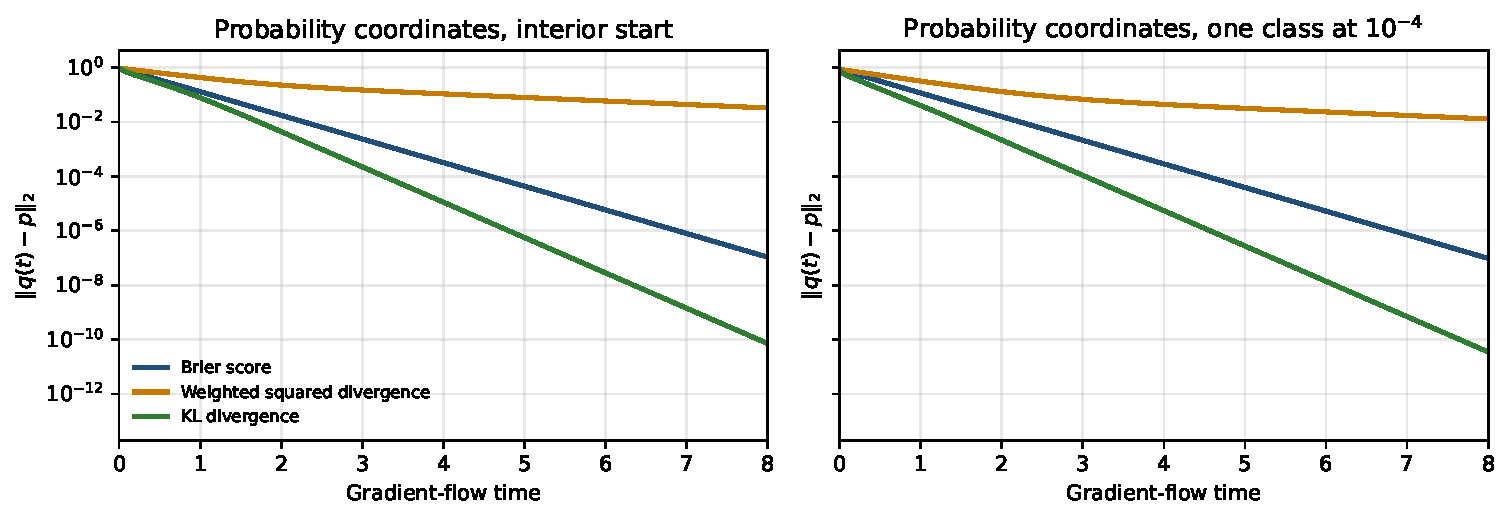
\includegraphics[width=\linewidth]{figures/flow_probability.pdf}
\caption{Euclidean projected gradient flow on the probability simplex, $p=(0.70,0.20,0.10)$.
Left: start at $(0.05,0.90,0.05)$.
Right: one coordinate starts at $10^{-4}$.
\textbf{Takeaway:} Kullback--Leibler divergence reaches distance $10^{-3}$ before the Brier score.
The weighted squared divergence is still near $10^{-2}$ at the right edge of each panel.}
\label{fig:prob-flow}
\end{figure}

From the interior start, the Brier score reaches distance $10^{-1}$, $10^{-2}$, and $10^{-3}$ at times $1.13$, $2.28$, and $3.43$.
Kullback--Leibler divergence reaches them at $0.91$, $1.72$, and $2.50$.
The weighted squared divergence reaches $10^{-1}$ at time $4.24$ and is at distance $0.0100$ at time $12$.
From the near-zero start the same three times for Kullback--Leibler divergence are $0.68$, $1.49$, and $2.26$.
The large derivative at a small coordinate shortens the early transient.
It does not create a slow mode.

These passage times are not the local times $0.50$, $3.38$, and $0.33$.
The linearization describes a neighborhood of $p$.
The ordering away from $p$ agrees with that neighborhood on these two starts: Kullback--Leibler divergence, then the Brier score, then the weighted squared divergence.

\section{Two different penalties at zero}
\label{sec:zero}

The question ``does log loss penalize zero the way the Brier score does?'' mixes two penalties.

The first is about symbols that did not occur.
Take $K=4$ and the observed symbol $0$, and compare
\[
q_{\mathrm{conc}}=(0.40,0.60,0,0), \qquad q_{\mathrm{spread}}=(0.40,0.20,0.20,0.20).
\]
Both assign probability $0.40$ to the observed symbol, so both have log loss $-\log 0.40=0.916$.
The Brier scores are $0.72$ and $0.48$.
The gap of $0.24$ is $\sum_{a\neq 0} q(a)^2$ under the two splits of the residual mass $0.60$.
Log loss has no term in that split.
The Brier score does.
For the uniform distribution on these four symbols, the weighted squared divergence of $q_{\mathrm{conc}}$ and $q_{\mathrm{spread}}$ is $0.0675$ and $0.0075$.
Kullback--Leibler divergence of $q_{\mathrm{spread}}$ is $0.0499$.
The forecast $q_{\mathrm{conc}}$ makes Kullback--Leibler divergence infinite, because two symbols in the support of $p$ have probability zero.
In that precise sense, log loss does not penalize unobserved symbols.

The second penalty is about a symbol that can occur and was given probability zero.
If $p(a)>0$ and $q(a)\to 0$, then $\KL(p\|q)\to+\infty$, while the Brier excess $\|q-p\|_2^2$ stays at most $2$.
Figure~\ref{fig:boundary} drives the rare coordinate of $p=(0.70,0.20,0.10)$ from $10^{-2}$ down to $10^{-8}$ and spreads the removed mass over the other two coordinates in the proportions of $p$.
At $10^{-2}$ the three excesses are $0.0134$ (Brier), $0.00432$ (weighted squared divergence), and $0.144$ (Kullback--Leibler).
At $10^{-8}$ they are $0.0165$, $0.00533$, and $1.517$.
The squared objectives have already met their finite limits.
Kullback--Leibler divergence is still climbing, by about $p(a)\log\bigl(1/q(a)\bigr)$ on the rare coordinate.

\begin{figure}[t]
\centering
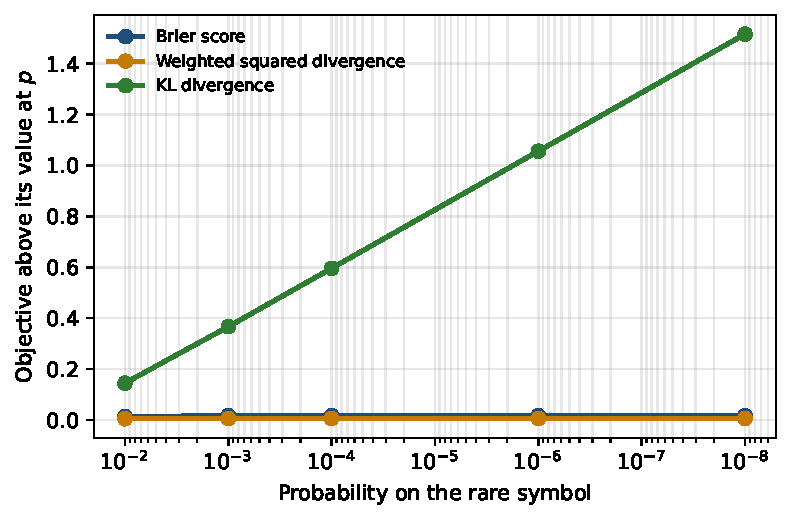
\includegraphics[width=0.78\linewidth]{figures/boundary_penalty.pdf}
\caption{Excess objective as the rare coordinate is driven from $10^{-2}$ to $10^{-8}$, for $p=(0.70,0.20,0.10)$.
The horizontal axis decreases to the right.
\textbf{Takeaway:} the Brier score and the weighted squared divergence level off.
Kullback--Leibler divergence keeps growing.
The growth is slow in the value and fast in the derivative.}
\label{fig:boundary}
\end{figure}

The derivative is the stability fact.
At rare probability $10^{-3}$ the Euclidean norm of the projected gradient is $0.255$ for the Brier score, $0.0947$ for the weighted squared divergence, and $80.9$ for Kullback--Leibler divergence.
At $10^{-8}$ those norms are $0.257$, $0.0957$, and $8.16\times 10^{6}$.
So $-\log 0=+\infty$ is the right description of the loss, and the practical failure mode in probability coordinates is the derivative $-p(a)/q(a)$, which is already large while the loss is still moderate.
The Brier score does not have this blow-up.
Its projected gradient stays near $0.26$ along this path.
The weighted squared divergence is flatter still, because the rare coordinate of its gradient carries a factor $p(a)$.

Locality does not contradict the barrier.
The scalar $-\log q(x)$ looks only at the observed coordinate, but the population objective is the average of that scalar.
Coordinate $a$ enters when $X=a$, with weight $p(a)$, and the contribution $p(a)\bigl(-\log q(a)\bigr)$ is steep when $q(a)$ is small.
The product of a rare symbol and a steep derivative is the eigenvalue $1/p(a)$ in \eqref{eq:hess-kl}, which is large.
The weighted squared divergence has the opposite product: its population gradient carries $p(a)$ and no $1/q(a)$, so the eigenvalue is proportional to $p(a)$ and the rare symbol is slow.

\section{Logit coordinates}
\label{sec:logits}

Let $q=\mathrm{softmax}(\theta)$.
The Jacobian of the softmax map satisfies $(J^\top v)_j = q(j)\bigl(v(j)-\langle q,v\rangle\bigr)$.
For expected log loss, $v=-p/q$ and this product collapses:
\begin{equation}
\label{eq:logit-kl}
\nabla_\theta R_{\log}(\mathrm{softmax}(\theta)) = q-p.
\end{equation}
The right-hand side is bounded by $1$ in every coordinate for any $\theta$.
Softmax never outputs an exact zero, so the loss is finite for every finite logit vector, and the gradient does not inherit the factor $1/q(a)$.
We checked \eqref{eq:logit-kl} analytically and against a finite difference of step $10^{-6}$ on a random four-symbol problem; the same finite-difference check was applied to the Brier and weighted logit gradients below, with error below $2\times 10^{-5}$.

The one-sample version of \eqref{eq:logit-kl} is $q-e_x$.
That vector does depend on every coordinate of $q$.
The scalar loss does not depend on how the residual mass is split, but the logit gradient subtracts nothing from an unobserved coordinate and then the softmax coupling moves probability off coordinates where $q(a)$ is large.
The penalty on unobserved symbols, which is absent from the scalar, is present in the parameterization people actually differentiate.

The Brier logit gradient does the opposite near zero.
With $v=2(q-p)$, the factor $q(j)$ in $J^\top v$ multiplies the whole coordinate.
A class with $q(j)\approx 0$ has almost no logit gradient, even if $p(j)$ is not small.
The weighted squared divergence has the same factor and an additional $p(j)$ inside $v$.

Figure~\ref{fig:logit-flow} integrates $\dot\theta=-\nabla_\theta R(\mathrm{softmax}(\theta))$ with an adaptive explicit Runge--Kutta method.
From $\theta=0$, so that $q$ starts uniform, Kullback--Leibler divergence reaches distance $10^{-3}$ at time $33.7$.
The Brier score reaches $10^{-2}$ at time $48.9$ and is at distance $0.00349$ at time $80$.
The weighted squared divergence reaches $10^{-1}$ at time $13.6$ and is at distance $0.0439$ at time $80$.
The order is the same as on the simplex.
The times are longer because the softmax Jacobian rescales the Euclidean gradient on $q$.

\begin{figure}[t]
\centering
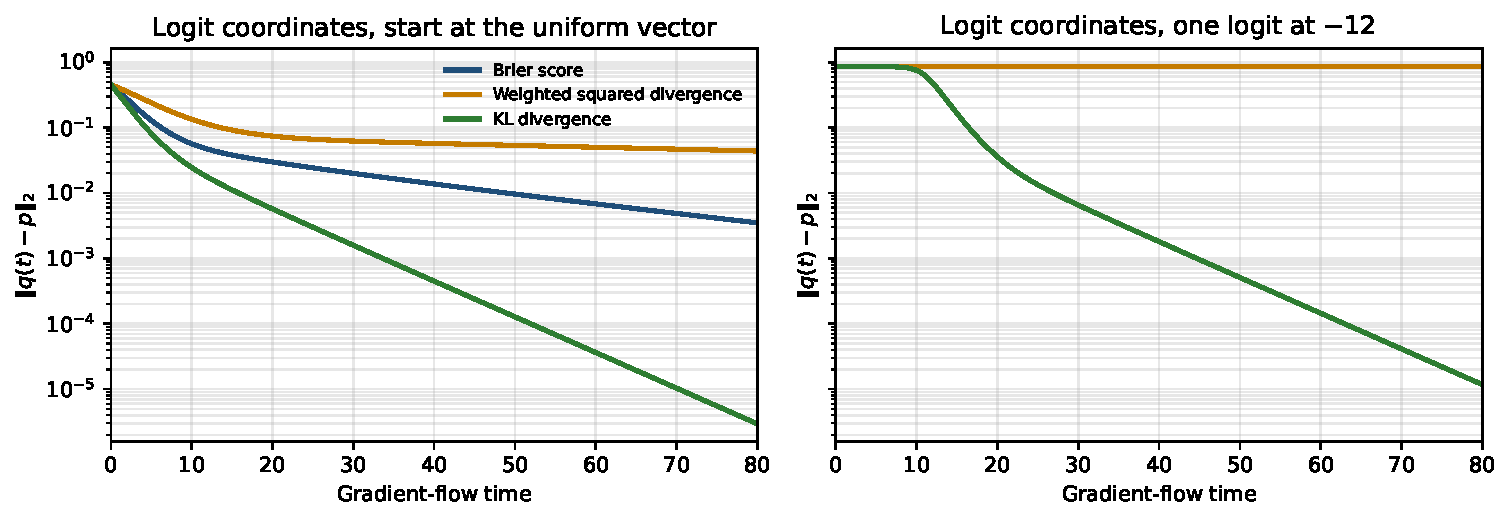
\includegraphics[width=\linewidth]{figures/flow_logit.pdf}
\caption{Gradient flow in softmax logit coordinates, $p=(0.70,0.20,0.10)$.
Left: every logit starts at $0$.
Right: the first logit starts at $-12$ and the others at $0$, so the first probability is $3.07\times 10^{-6}$.
\textbf{Takeaway:} from a collapsed logit, Kullback--Leibler divergence reaches distance $10^{-3}$ at time $44.7$.
The Brier score and the weighted squared divergence are still at distance $0.857$ and $0.873$ at time $80$.}
\label{fig:logit-flow}
\end{figure}

The right panel is the stability comparison.
At the collapsed start the logit gradients on the collapsed coordinate are $-0.700$ for Kullback--Leibler divergence, $-6.5\times 10^{-6}$ for the Brier score, and $-3.3\times 10^{-6}$ for the weighted squared divergence.
Kullback--Leibler divergence reaches distance $10^{-1}$, $10^{-2}$, and $10^{-3}$ at times $16.4$, $26.9$, and $44.7$, and is at distance $1.17\times 10^{-5}$ at time $80$.
The other two objectives never reach distance $10^{-1}$.
Their terminal distances, $0.857$ and $0.873$, sit next to the initial distance $0.860$.
On this horizon a class that has collapsed in logit coordinates is revived by log loss and is not revived by the Brier score.

Making log loss ``as stable as the Brier score'' by adding a penalty on unobserved symbols would be answering a different instability from the one the Brier score has.
In probability coordinates the Brier gradient is the bounded one and the log-loss gradient is not.
In logit coordinates the log-loss gradient is the bounded one, and it is the Brier gradient that vanishes on a collapsed class.

\section{What cannot be repaired while staying local and proper}
\label{sec:repair}

A smooth local proper score on $K\ge 3$ symbols is an affine image of log loss \citep{bernardo1979,mit67800}.
Every such score tends to $+\infty$ as $q(x)\to 0$, and its probability-space derivative in the observed coordinate is $-A/q(x)$, which is unbounded on $\Delta$.
Adding a penalty that depends on $q(a)$ for $a\neq x$ leaves the local class.
The Brier score is that departure, with the unobserved sum $\sum_{a\neq x} q(a)^2$ matched to the observed square so that Proposition~\ref{prop:brier-pop} holds.
There is no third option that is smooth, local, proper, and free of the barrier.

We measured two attempts to keep a local formula and soften the barrier.
Both use $p=(0.70,0.20,0.10)$ and a sequential least-squares solver from $10$ starts.
The loss at the reported vector is at most the loss at $p$.

The first attempt adds a local square penalty, $R_{\log}(q)+\lambda\, \mathbb{E}\bigl[(1-q(X))^2\bigr]$.
At $\lambda=0$ the minimizer is $p$, to distance $2.7\times 10^{-9}$.
At $\lambda=1$ the distance is $0.0274$, with $q=(0.722,0.193,0.085)$.
At $\lambda=10$ the distance is $0.0846$, with $q=(0.762,0.195,0.043)$.
The same multiple of the Brier score, $R_{\log}+\lambda R_{\BS}$, stays within distance $10^{-8}$ of $p$ at $\lambda=0$, $1$, and $10$.
A sum of proper scores with nonnegative weights is proper.
A sum of log loss and the local square score is local and is not proper.

The second attempt clips the logarithm, $\mathbb{E}\bigl[-\log\max\bigl(q(X),\varepsilon\bigr)\bigr]$.
At $\varepsilon=10^{-8}$ and at $\varepsilon=10^{-3}$ the minimizer is $p$, to distance below $10^{-7}$.
At $\varepsilon=0.05$, which is below the smallest coordinate $p(a)=0.10$, the minimizer is $(0.778,0.222,0)$, at distance $0.129$, and its clipped loss is $0.776$ against $0.802$ at $p$.
At $\varepsilon=0.15$ the minimizer is a point mass on the largest coordinate, at distance $0.374$.
Clipping does not have to cross $p(a)$ before it moves the minimizer.
Once a coordinate falls below $\varepsilon$, that coordinate's derivative vanishes and the remaining problem can prefer the clipped face.

A third construction keeps propriety and changes the target.
The smoothed distribution $(1-\alpha)p+\alpha\,\mathrm{Unif}$ is the minimizer of expected log loss for that smoothed distribution, not for $p$.
At $\alpha=0.10$ its Euclidean distance to $p$ is $0.0455$.
That bias is the price of pulling the target off the boundary.
It is proper for the smoothed distribution.
It is not a repair of log loss for $p$.

\section{One-sample updates}
\label{sec:sgd}

The population flows use $p$ in the vector field.
A one-sample update cannot do that for the weighted squared divergence, because \eqref{eq:wd} is not an expectation of a function of $(X,q)$ alone.
Log loss and the Brier score can.
In logit coordinates the one-sample gradients are $q-e_X$ and $J^\top\bigl(2(q-e_X)\bigr)$.

Figure~\ref{fig:sgd} shows $40$ paired seeds on $p=(0.70,0.20,0.10)$, each seed an independent sequence of $8000$ outcomes.
The step at update $t$ is $t^{-1/2}$, shared across objectives.
The weighted curve is the population logit gradient of $\WD$, stepped on the same schedule and independent of the seed.
The band is the mean plus or minus $1.96$ standard errors across the $40$ seeds.
The weighted curve has no band.

\begin{figure}[t]
\centering
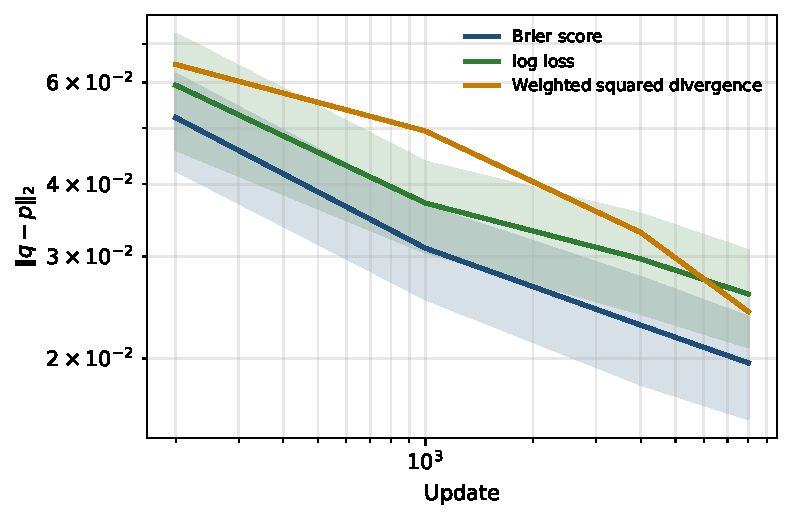
\includegraphics[width=0.72\linewidth]{figures/sgd_logit.pdf}
\caption{Logit updates with step $t^{-1/2}$, $p=(0.70,0.20,0.10)$.
Log loss and the Brier score use one sample per update, on the same $40$ sequences.
The weighted squared divergence uses its population gradient.
The band is the mean $\pm 1.96$ standard errors.
\textbf{Takeaway:} under this shared diminishing step the two one-sample scores stay close.
At $8000$ updates the paired gap is $0.0062\pm 0.0009$, with the Brier score closer.
That gap is small next to the collapsed-logit separation in Figure~\ref{fig:logit-flow}.}
\label{fig:sgd}
\end{figure}

At $200$, $1000$, $4000$, and $8000$ updates the Brier distances are $0.0522\pm 0.0050$, $0.0310\pm 0.0029$, $0.0228\pm 0.0024$, and $0.0196\pm 0.0020$.
The log-loss distances are $0.0594\pm 0.0068$, $0.0371\pm 0.0034$, $0.0297\pm 0.0030$, and $0.0258\pm 0.0025$.
The paired difference, log loss minus Brier, is $0.0062\pm 0.0009$ at the last checkpoint.
The shared step is a larger fraction of a typical log-loss update than of a typical Brier update, because the Brier logit gradient carries a factor $q(j)$.
The population flows in Sections~\ref{sec:rates} and~\ref{sec:logits} are the step-free comparison.
This figure is evidence that one-sample noise does not reverse the conclusion of Section~\ref{sec:zero}: both proper scores descend, and the dramatic separation appears when a coordinate has collapsed, not in the average of ordinary updates.

\section{Limitations}

The forecast $q$ is the distribution itself.
There are no covariates and no restricted parametric family.
In a restricted family the three population minimizers can differ even though each proper objective would recover $p$ if $p$ were in the family.
The histogram identity in Section~\ref{sec:identity} would then be false.

The probability-space flow uses the Euclidean metric and projection onto $\Delta$.
The logit flow uses the Euclidean metric on $\theta$.
Neither is the Fisher--Rao metric.
Natural gradient for log loss would replace \eqref{eq:logit-kl} by a different parameterization of the same objective; we do not claim a rate for it.

The weighted squared divergence in the one-sample figure is an oracle step.
It is there so the three vector fields can share a step, not as a method one can run from $x$ alone.

Passage times depend on the start.
We report the interior start used in the earlier comparison, a near-zero start, the uniform logit vector, and one collapsed logit.
The local rates do not depend on the start, and the matrix-exponential check on those rates does not either.

The clipped-log and penalized-log minimizers are numerical.
Each reported vector beats $p$ on the objective that produced it, or matches $p$ to the distance stated.
We do not claim a closed form for the clipped problem.

The flows use one skewed distribution, $p=(0.70,0.20,0.10)$, plus the exact uniform and binary rates in Section~\ref{sec:rates}.
The code is \texttt{run\_kl\_comparison.py} in this directory, seed $0$, NumPy $2.2.6$ and SciPy $1.16.3$.
The expectation identities in Section~\ref{sec:defs} are checked by \texttt{run\_expectation\_identity.py}, including a Monte Carlo average of $10^5$ draws.

\section{Conclusion}

The weighted squared divergence and Kullback--Leibler divergence are both expectations under $p$ of a discrepancy between $p(X)$ and $q(X)$, with discrepancies $(p(X)-q(X))^2$ and $\log p(X)-\log q(X)$.
The Brier score, the weighted squared divergence, and Kullback--Leibler divergence are minimized at the true distribution.
They do not approach it at the same local rate.
The weighted squared divergence is slower on rare symbols, by a factor $6.77$ on the slow mode for $p=(0.70,0.20,0.10)$, because its gradient is multiplied by $p(a)$.
Kullback--Leibler divergence is faster on those symbols, because its Hessian is $\mathrm{diag}(1/p)$.
The local square score, which is what a one-hot substitution makes of the weighted squared divergence, is a different objective and is not proper once the alphabet has three or more symbols.

Log loss is local, and that does not make it slow.
Locality means the scalar $-\log q(x)$ ignores the split of the residual mass; the Brier score does not.
The barrier $-\log 0=+\infty$ is a penalty on putting zero probability on a symbol that can occur, and it is a stronger penalty than the Brier score's finite square, not a weaker one.
The derivative that comes with the barrier is large exactly where a coordinate is too small, which is the opposite of a slow direction.

In logit coordinates that derivative becomes $q-p$, which is bounded, and it revives a class whose logit sits at $-12$.
On that same horizon the Brier score does not revive it: the softmax Jacobian multiplies the Brier gradient by the collapsed probability.
A smooth local proper score cannot avoid the barrier, because every such score is an affine image of log loss.
Adding a local square penalty, or clipping the logarithm at a floor below the smallest true probability, moves the minimizer.
Adding the Brier score itself does not.
The stable proper score that penalizes unobserved symbols in the scalar loss is the Brier score, and it is not local.
The stable parameterization of the local proper score is the softmax, and it does not need an extra unobserved-symbol term.

\bibliographystyle{tmlr}
\bibliography{main}

\end{document}
